\documentclass{article}
\usepackage{indentfirst}
\usepackage[margin={1in}]{geometry}
\usepackage{graphicx}
\usepackage[section]{placeins}
\usepackage{amsmath}
\usepackage[T1]{fontenc}

\graphicspath{ {/} }

\begin{document}

\title{Team One Project Proposal}
\author{John~Ure, Maria~Walshe, and Matthias~Guenther}
\date{\today}
\maketitle

\clearpage

\section*{Domain Description}{

	We are proposing to design, model, and build a speed-reading trainer for those who might want to improve their reading speed. The splash screen on startup will allow the user to create a new user or access a previously stored user.\\

	The software will contain profiles for multiple users. Each user will consist of a name, a list of documents which will contain the last 10 text documents they have opened, and an interface object that will contain their current UI options such as pointer type, preferred font, and speed setting in WPM.\\

	Each user will be associated with a unique catalog of files; each such document will contain its physical location on disk and statistics as to the user's performance for that specific document. In the GUI, once the user profile is selected, document physical locations will show on the left of the panel. Each physical location can be overridden with a user-specified document name for ease of use. The interface will also open the text body of the document and display the current user statistics associated with that document.\\

	The user may either manually set a new bookmark location with the scroll bar and mouse click, or resume from the current location setting. The bookmarked word will display with the pointer type selected by the user. The highlight block will be the default type, but the user may change this to either the underline or the caret symbol if they choose. Pressing \textbf{spacebar} will begin traversing the text at the selected speed, which the user may change at any time using $\boldsymbol{<}$ or $\boldsymbol{>}$ (or their lowercase equivalents).\\

	Once the document is paused, the user may choose to save their place, open a new document, or reset their statistics for this document by selecting the \textit{File} menu item.\\

	The user may also switch to another existing profile or create a new profile (and switch to that one) from the \textit{User} menu item.\\

	From the \textit{Options} menu, the user may change their speed setting, display font, and pointer type (either word highlight, underline, or pointer arrow).\\
}

\clearpage

\section*{Constraints Analysis}{

	For the purposes of this project, the software will only support plain-text files. If it were to be distributed to end users on a large scale, it would be important to add support for other file types such as epub, doc/docx, rtf, and compatible types of pdf.\\

	The software will assume documents use the Latin alphabet, preventing its use on many foreign languages. That said, some of the omitted languages have fundamental differences in how they are read, e.g. Mandarin, where characters represent entire words. Such languages might or might not be conducive to the same form of speed-reading training in the first place.\\
}

\clearpage

\section*{Domain Analysis}{

	Below is the UML that is proposed at this point in the design. While it may change, it is representative of what we intend to build.\\

	\begin{figure}[!htb]
		\centering
		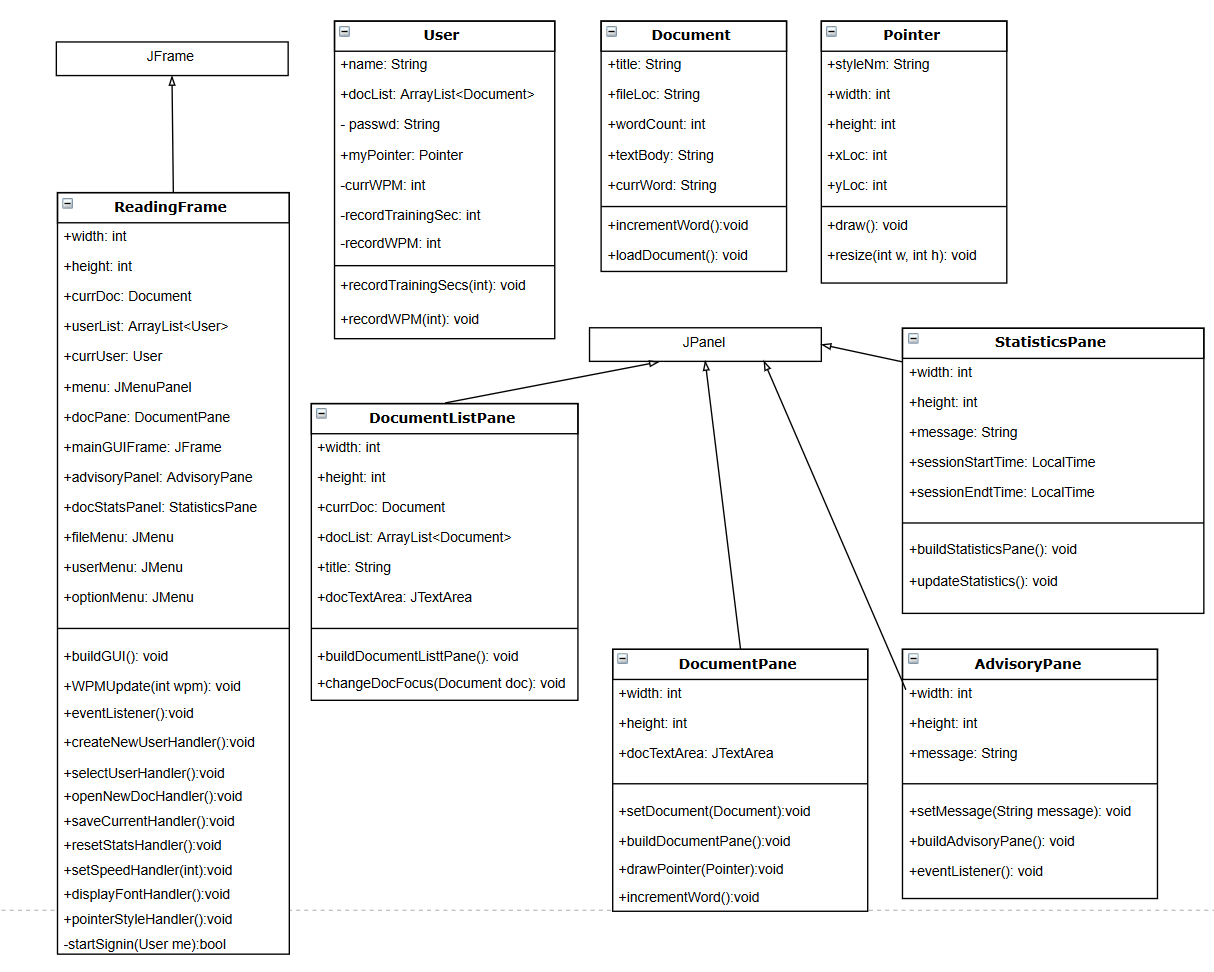
\includegraphics[scale=.5]{UMLDiagram.png}
		\label{fig:fig1}
		\caption{UML Diagram}
	\end{figure}
}

\clearpage

\section*{Interaction Analysis}{

	The following screen will display on startup, allowing the creation of a new user or the loading of an existing one.\\

	\begin{figure}[!htb]
		\centering
		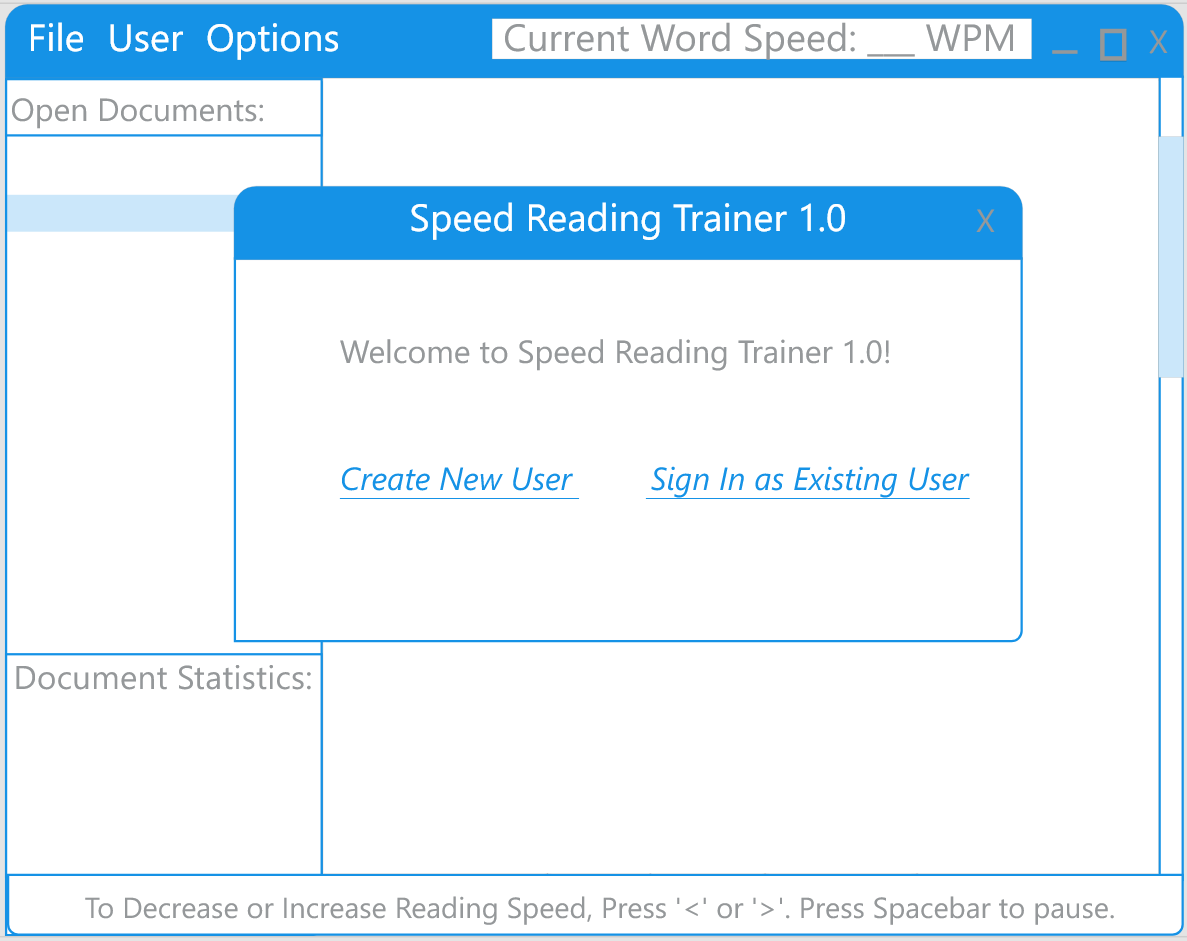
\includegraphics[scale=.7]{StartupSplashScreen.png}
		\label{fig:fig2}
		\caption{Startup Splash Screen}
	\end{figure}

	\clearpage

	The main interface is displayed below, including the sidebar of recent documents, the user statistics, and the current document.\\

	\begin{figure}[!htb]
		\centering
		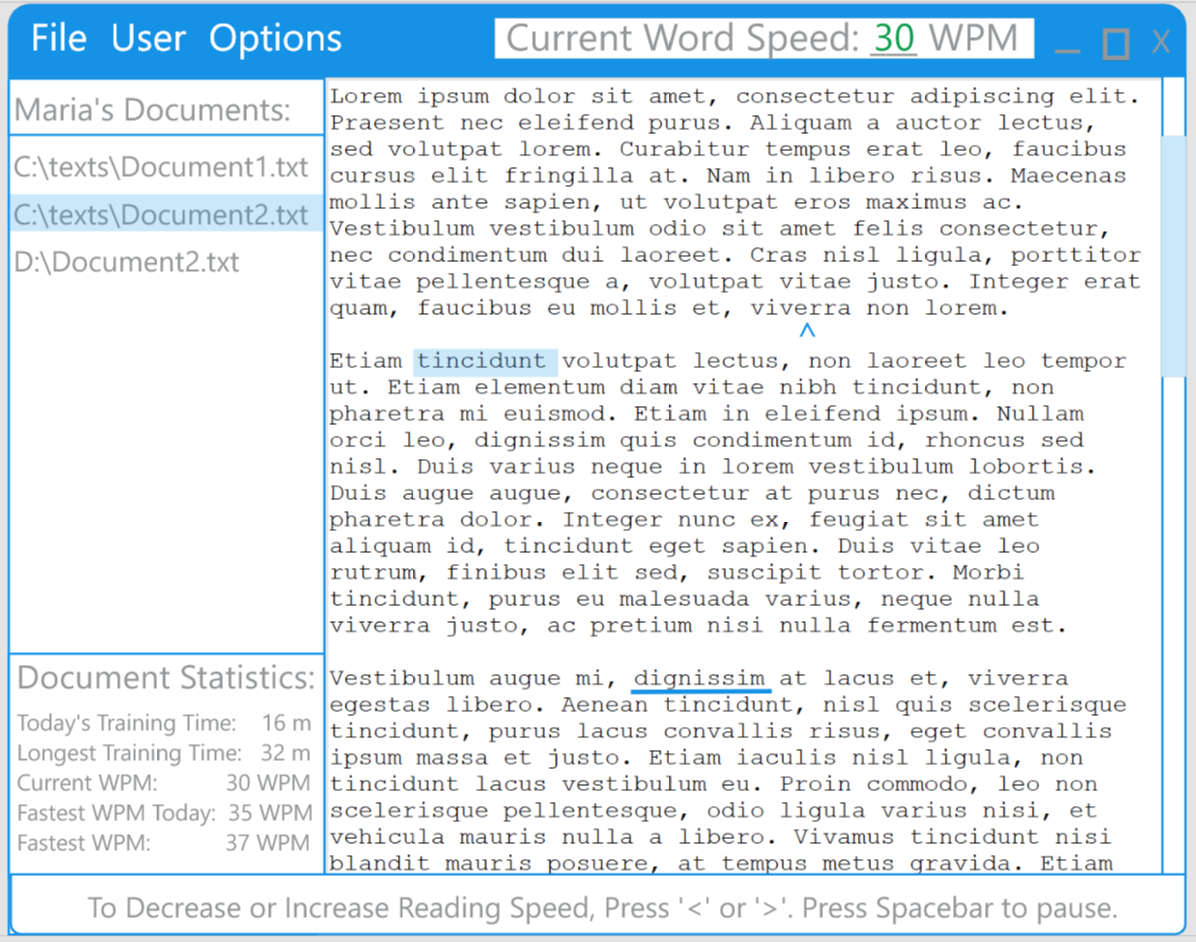
\includegraphics[scale=.7]{MainInterface.png}
		\label{fig:fig3}
		\caption{Main Interface}
	\end{figure}

	\clearpage

	The \textit{File} menu contains options for opening a document, saving one's place in the current document, and resetting the statistics stored for that document.\\

	\begin{figure}[!htb]
		\centering
		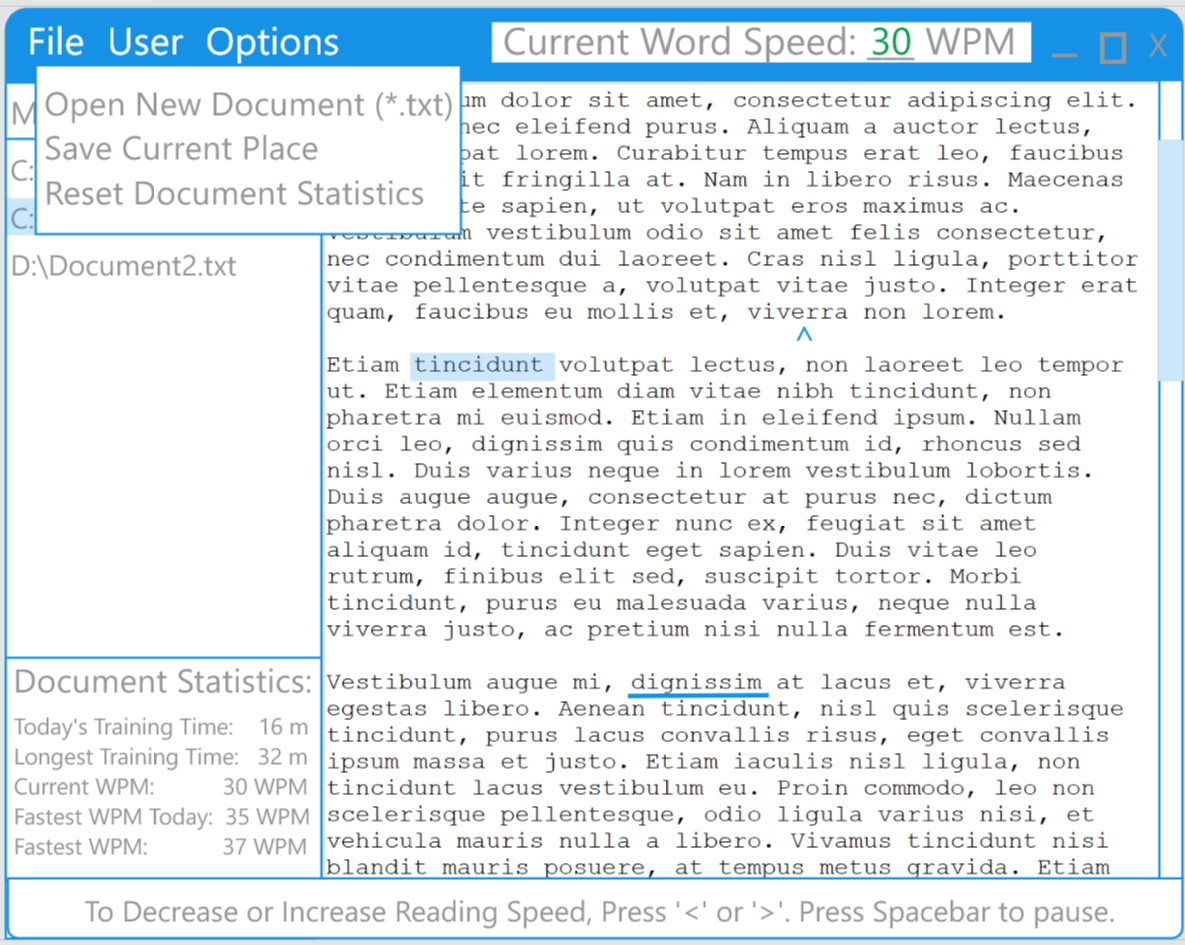
\includegraphics[scale=.7]{FileMenu.png}
		\label{fig:fig4}
		\caption{File Menu}
	\end{figure}

	\clearpage

	The \textit{User} menu contains options for switching profiles. The target profile can already exist or can be created on the spot.\\

	\begin{figure}[!htb]
		\centering
		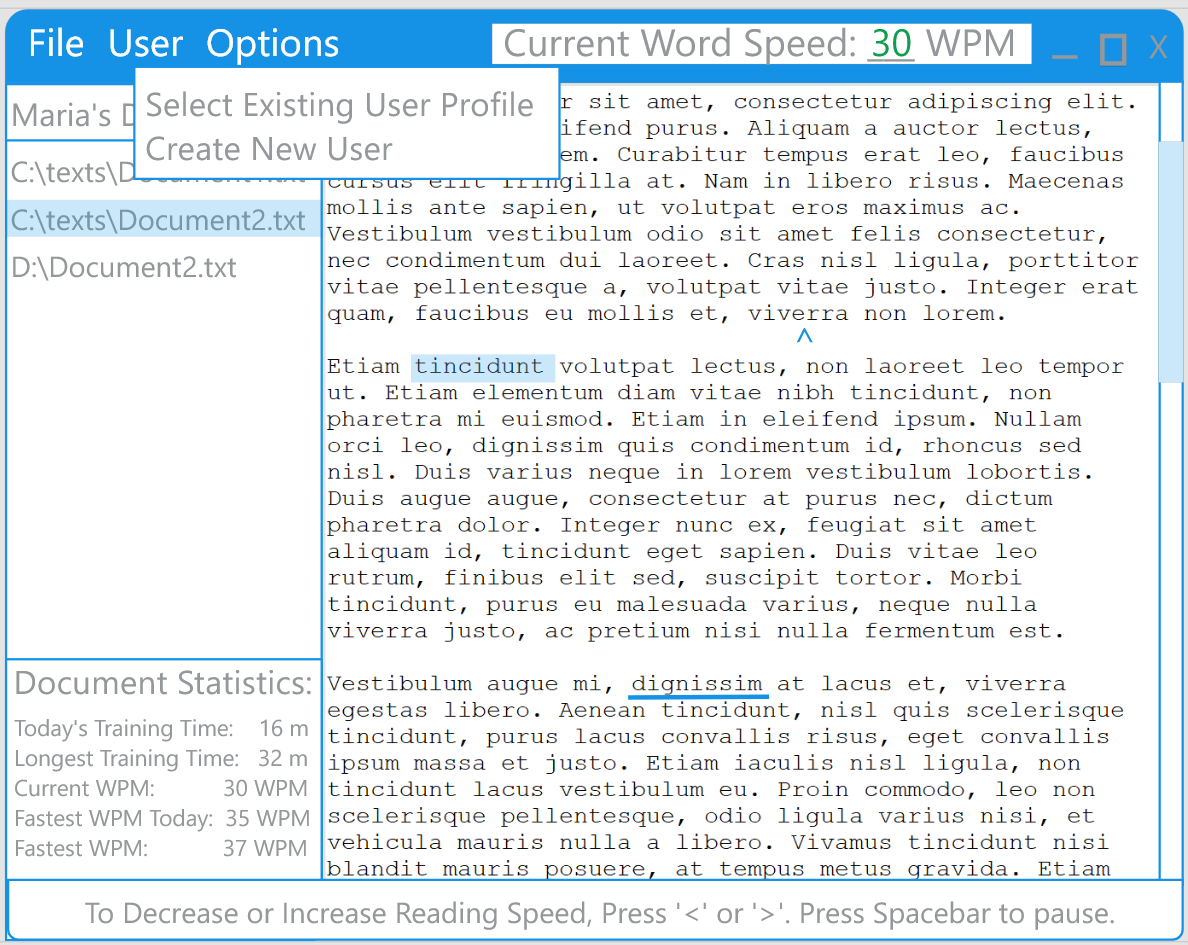
\includegraphics[scale=.7]{UserMenu.png}
		\label{fig:fig5}
		\caption{User Menu}
	\end{figure}

	\clearpage

	The \textit{Options} menu contains settings for reading speed, font formatting, and the type of marker used to indicate the user's current place in the document.\\

	\begin{figure}[!htb]
		\centering
		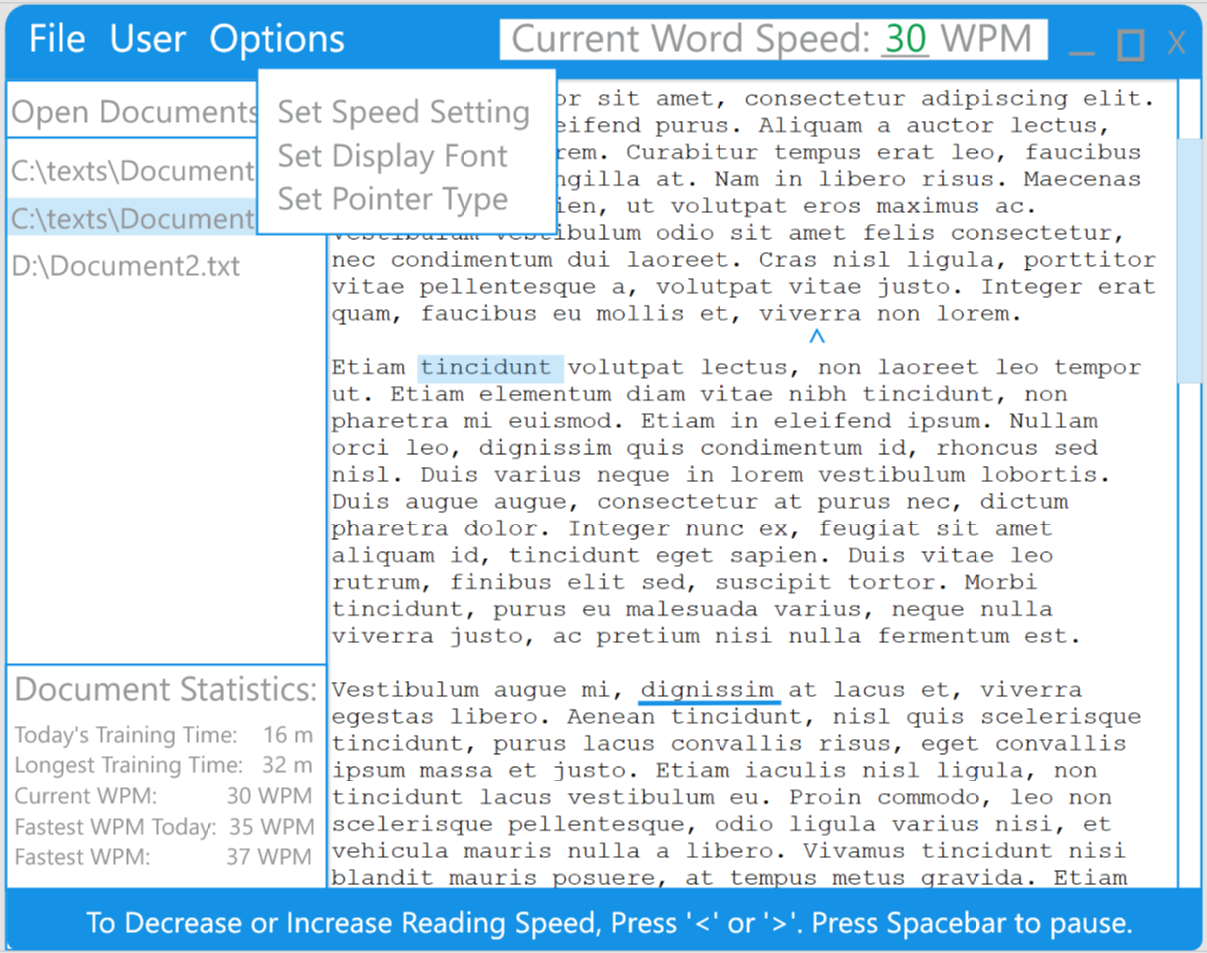
\includegraphics[scale=.7]{OptionsMenu.png}
		\label{fig:fig6}
		\caption{Options Menu}
	\end{figure}

	\clearpage

	Below is a flowchart for user interaction with the software.\\

	\begin{figure}[!htb]
		\centering
		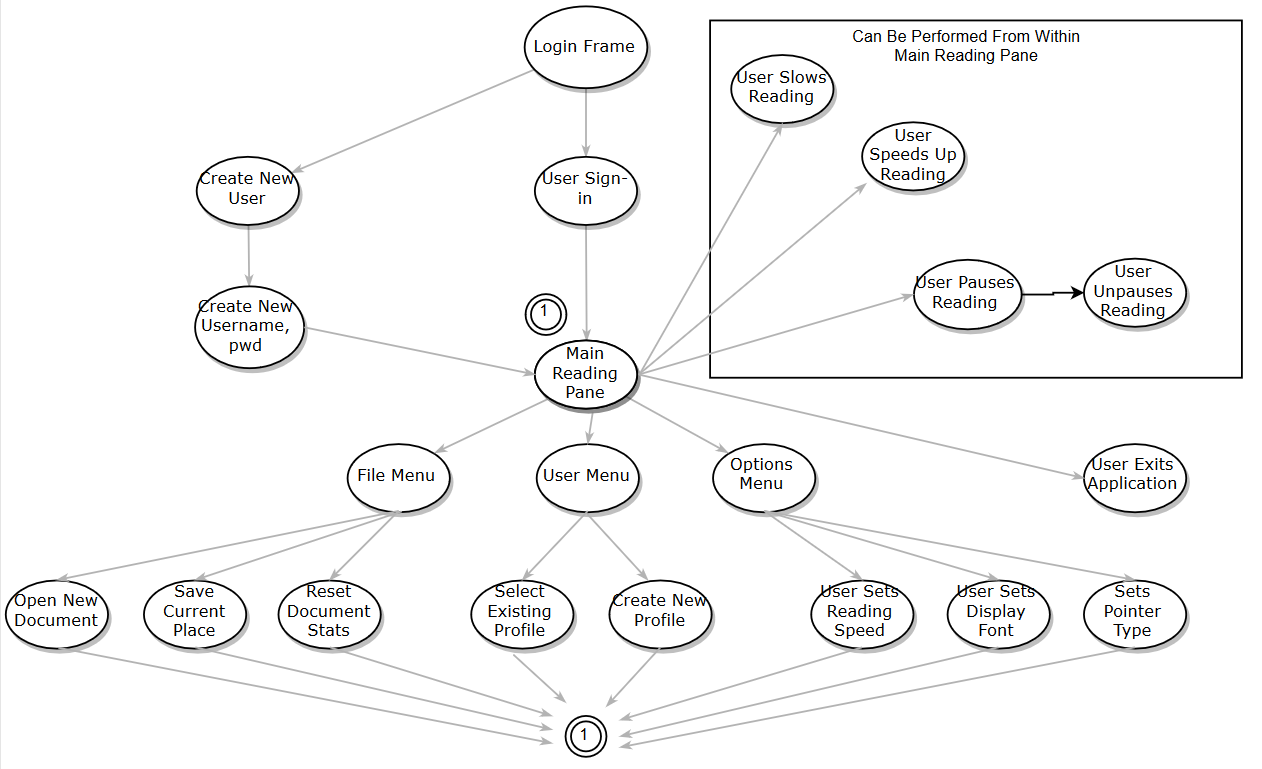
\includegraphics[scale=.5]{UserBehaviorModel.png}
		\label{fig:fig7}
		\caption{User Behavior Model}
	\end{figure}
}

\clearpage

\section*{Plan of Work}{
	
	The team will meet each week at 4:00 pm on Fridays from October 27$^\text{th}$ to December 1$^\text{st}$. Although work will largely be shared between team members, the primary members in charge of each milestone are outlined below.\\

	\begin{table}[!htb]
		\centering
		\begin{tabular}{| c | c | c | c |}
			\hline
			\textbf{Milestone}	&	\textbf{Start Date}	&	\textbf{End Date}	&	\textbf{Primary Members}	\\
			\hline
			% Initial stage:
			Preliminary GUI		&	10/27/17			&	11/03/17			&	John Ure					\\
			Document handling	&	10/27/17			&	11/03/17			&	Maria Walshe				\\
			User handling		&	10/27/17			&	11/03/17			&	Matthias Guenther			\\
			\hline
			% Intermediate stage:
			File I/O			&	11/03/17			&	11/10/17			&	Maria Walshe				\\
			GUI finalization	&	11/03/17			&	11/24/17			&	Matthias Guenther, John Ure	\\
			\hline
			% Final stage:
			Unit testing		&	11/24/17			&	11/24/17			&	Distributed	by component	\\
			Integration			&	11/24/17			&	11/24/17			&	All							\\
			Final testing		&	11/24/17			&	12/01/17			&	All							\\
			\hline
			% Overall:
			Overall timeline	&	10/27/17			&	12/01/17			&	All							\\
			\hline
		\end{tabular}
		\label{tbl:tbl1}
		\caption{Project Timeline}
	\end{table}
}

\end{document}